%
% File naaclhlt2010.tex
%
% Contact: nasmith@cs.cmu.edu

\documentclass[11pt,letterpaper]{article}
\usepackage{naaclhlt2010}
\usepackage{times}
\usepackage{latexsym}
\usepackage{graphicx}
\setlength\titlebox{6.5cm}    % Expanding the titlebox

\newlength{\rhwidth}
\newcommand{\planaction}[3]{
\begin{minipage}{.5\textwidth}
\footnotesize
\setlength{\rhwidth}{.5\textwidth}
\addtolength{\rhwidth}{2.0cm}
{#1:}

\noindent \hspace{.2cm} \begin{minipage}{1.5cm}{Precond:}\end{minipage}\begin{minipage}[t]{\rhwidth} #2 \end{minipage}

\noindent \hspace{.2cm} \begin{minipage}{1.5cm}{Effect:}\end{minipage} \begin{minipage}[t]{\rhwidth}\ #3 \end{minipage}
\end{minipage}
}

\newcommand{\cplanaction}[4]{
\begin{minipage}{.5\textwidth}
\footnotesize
\setlength{\rhwidth}{.5\textwidth}
\addtolength{\rhwidth}{2.0cm}
{#1:}

\noindent \hspace{.2cm} \begin{minipage}{1.5cm}{Precond:}\end{minipage}\begin{minipage}[t]{\rhwidth} #2 \end{minipage}

\noindent \hspace{.2cm} \begin{minipage}{1.5cm}{Effect:}\end{minipage} \begin{minipage}[t]{\rhwidth} #3 \end{minipage}

\noindent \hspace{.2cm} \begin{minipage}{1.5cm}{Cost:}\end{minipage} \begin{minipage}[t]{\rhwidth} \ensuremath{#4} \end{minipage}
\end{minipage}
}



\title{Sentence Generation as Planning with Probabilistic LTAG\\
%\Thanks{}
}

\author{Daniel Bauer\\
  Columbia University\\
  New York, NY, USA\\
  {\tt bauer@cs.columbia.edu} 
  \And
  Alexander Koller\\
  Saarland University\\
  Saarbr\"{u}cken, Germany\\ 
  {\tt koller@mmci.uni-saarland.de}}

\date{}

\begin{document}
\maketitle
\begin{abstract}
Our work merges combined sentence planning and surface realization using 
{\sc ltag} and statistical generation. This makes it possible to address
integrated sentence generation with large, treebank induced grammars for
the first time.
\end{abstract}

\section{Introduction}
\label{sec:introduction}


The International Planning Competition (IPC)\footnote{See
\url{http://ipc.icaps-conference.org/}.} recently celebrated its 10-year
anniversary in 2008. During this time, six instances of the IPC have been
run, each of which has helped drive the development of new planning
technology, by providing a regular forum for showcasing the latest trends
in planner design, domain description languages, and challenging planning
domains. Given the absence of a competition in 2010---breaking the
competition's established two year cycle for the first time since its
inception---we feel the time is right to revisit the structure of the
existing IPC, and suggest a new direction for the competition in the
future.

This paper proposes a new direction for the IPC, building on the strength
of previous competitions and inspired by competitions in other research
communities. Most notably, we envision an interactive and user-centric
%potentially more wide-ranging
competition, focused around a novel online infrastructure featuring:
%Most notably, we envision a more interactive and potentially more
%wide-ranging competition featuring:
%
\begin{itemize}
\item A ``rolling'' competition format with community-initiated track and
problem specifications,

\item Continuous evaluation of contributed planners on competition
problem sets, with real-time access to performance data generated on a
common hardware platform, and

\item A centralised repository offering researchers access to the latest
domains and planners, and a social networking forum for community news,
discussion, and interaction.
\end{itemize}

Thus, while previous instances of the IPC have traditionally been
event-based competitions, scheduled at regular intervals, we propose an
ongoing competition as a permanent fixture for the planning community. In
particular, members of the community would be able to upload new planners
and problem domains to a central competition server that continually
re-evaluates planners and generates performance data. Up-to-the-minute
results would be centrally available, while more formal competitions could
be ``run'' at regular intervals by producing snapshots of current planners
and problems. 

From a technical point of view, it is important to note that such an
idea would not have been practical ten years ago during the time of
the first IPC. It is only recently, due to advances in computing
hardware, network bandwidth, and available software infrastructure,
that a scenario such as this is now feasible. Even so, our proposed
infrastructure nevertheless presents some technical challenges that
must be addressed (e.g., security, accessibility, maintenance,
etc.). However, we believe that for the most part, solutions to these
problems can already be found by looking at similar (although smaller
scale) competition efforts in the wider research community.

Most importantly, we believe this proposal offers significant benefits to
the competition stakeholders: organisers, participants, and the wider
planning community. Furthermore, since much of the infrastructure we
describe is not tied to a specific research area, attempts to establish
similar competitions could benefit from this approach, leading to joint
ventures with research fields beyond planning---and the
possibility of future inter-disciplinary challenges.

%RP: Alexander's first couple sentences in the next section are a good lead
%in to the content of the paper. I don't think we need much or anything
%as a transition here, especially if we're short on space.

%In the remainder of the paper we outline our proposal for a new competition
%infrastructure, and the benefits we believe this approach could bring to
%the planning community and beyond.


%%% Local Variables: 
%%% mode: latex
%%% TeX-master: "main"
%%% End: 

\section{Related Work} \label{sec:related}


\todo{Note: This is \emph{not} search (compare
\cite{DBLP:conf/ijcai/BohnetD05}). }


\begin{figure}
  \centering
  \begin{tabular}{l|l}
    GRE algorithm & DL variant \\ \hline
    \newcite{Dale1995} & conjunctions of atoms \\
    \newcite{deemter01:_gener_refer_expres} & propositional logic \\
    \newcite{dale91:_gener_refer_expres_invol_relat} & \el \\
    \newcite{Krahmer2003} & \el \\
    \newcite{kelleher06:_increm_gener_of_spatial_refer} & \el \\
    \newcite{gardent02:_gener_minim_defin_descr} & \alc
  \end{tabular}
  \caption{DL variants used by different GRE algorithms.}
  \label{fig:related}
\end{figure}

The view of GRE as a problem of computing DL concepts allows us to
organize existing approaches to GRE with respect to the logical
connectives of DL which they can use in the referring expressions they
generate.  This is summarized for some approaches in
Fig.~\ref{fig:related}.  At the most unexpressive end of the spectrum,
\newcite{Dale1995} only generate referring expressions that correspond
to conjunctions of atomic concepts.
\newcite{deemter01:_gener_refer_expres} adds the other propositional
connectives (negation and disjunction) to this, whereas
\newcite{dale91:_gener_refer_expres_invol_relat} and its successors
\cite{Krahmer2003,kelleher06:_increm_gener_of_spatial_refer} add
existential quantifiers.  The graphs used by \newcite{Krahmer2003} can
also be seen as concepts of \el\ that are only satisfied at the points
at which they can be embedded.
\newcite{gardent02:_gener_minim_defin_descr} combines these strands
into an algorithm which computes arbitrary concepts in \alc. \todo{Is
  this really what Claire does?}

In this paper, we have presented two algorithms for concepts in \el\
and \alc.  These algorithms compute referring expressions for all
individuals in the domain at once, and thus there is no danger of
infinite regress.  Other approaches for \el\ and higher logics
typically have to invest some effort into avoiding infinite regress --
e.g.\ by requiring that no edge may be used twice
\cite{dale91:_gener_refer_expres_invol_relat} or that no node may be
used twice \cite{kelleher06:_increm_gener_of_spatial_refer}.  The
graph-based algorithm by \newcite{Krahmer2003} avoids infinite regress
with similar ease as our algorithms -- adding an edge to a subgraph
twice doesn't change the subgraph --, but this comes at the price of
NP-complete complexity.

Because they compute referring expressions for all individuals in the
domain together, our algorithms will be strongest in static settings,
such as the generation of descriptions for museum exhibits, in which
the individuals and their properties don't change much.  Nevertheless,
they remain fast enough for real-time use in dynamic settings.
Another advantage that recent algorithms for relational REs
\cite{Krahmer2003,kelleher06:_increm_gener_of_spatial_refer} have over
ours is that they can take weights and salience into account.  How
this could be incorporated into our algorithms is an interesting
question for future research.


%%% Local Variables: 
%%% mode: latex
%%% TeX-master: "dl-gre-08"
%%% End: 
 % Related work
\section{Sentence generation as planning}
\label{sec:crisp}


We consider a planning domain that comes up in the generation of
natural language sentences based on tree-adjoining grammar (TAG;
\cite{joshi;etal1997}).  This is a standard problem in computational
linguistics, which we sketch by example; see
\cite{Stone2003a,KolSto07} for details.

% \begin{figure}
%   \centering
%   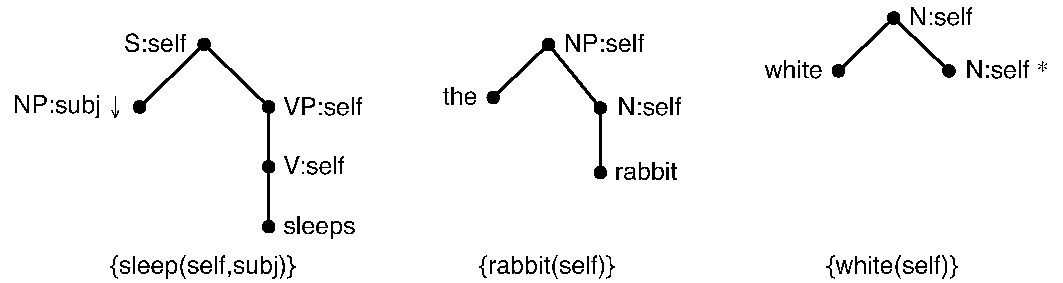
\includegraphics[width=0.75\columnwidth]{pic-grammar}
%   \caption{An example grammar in the sentence generation domain.}
%   \label{fig:white-rabbit-sleeps-grammar}
% \end{figure}

\begin{figure}
  \centering
  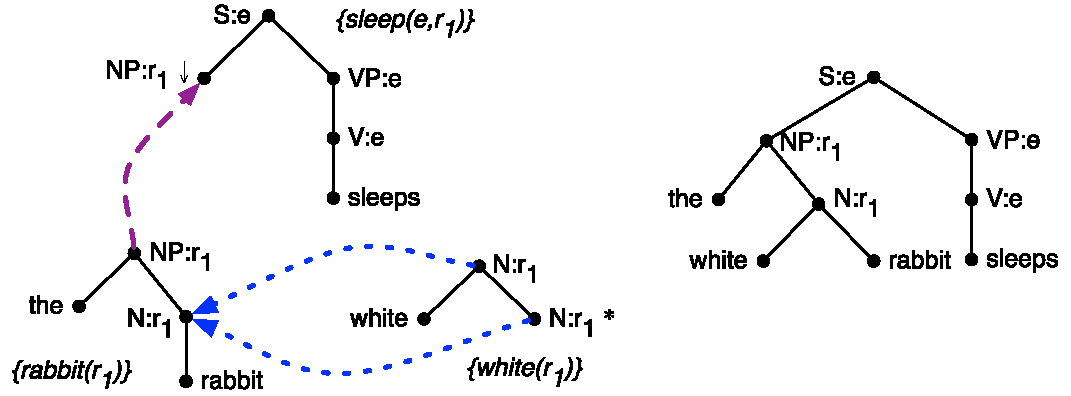
\includegraphics[width=1\columnwidth]{pic-derivation}
  \caption{Derivation of ``The white rabbit sleeps.''}
  \label{fig:white-rabbit-sleeps-deriv}
\end{figure}

A TAG grammar consists of a finite set of \emph{elementary trees},
each of which contains one or more words; the left of
Fig.~\ref{fig:white-rabbit-sleeps-deriv} shows three trees for ``the
rabbit'', ``sleeps'', and ``white''.  Trees can be combined using the
operations of \emph{substitution} (purple dashed arrow in the figure)
and \emph{adjunction} (blue dotted arrows) to form larger trees.
The end result of a grammatically correct derivation is a tree all of
whose leaves are labeled with words, as on the right of
Fig.~\ref{fig:white-rabbit-sleeps-deriv}. We can read off a sentence
from such a tree from left to right.

To use TAG grammars for generation \cite{Stone2003a}, we assume a set
of ground atoms expressing the information we want the sentence to
convey, such as $\{\mathsf{sleep}(e,r_1)\}$, and a knowledge base that
contains all ground atoms we know to be true; say,
$\{\mathsf{sleep}(e,r_1), \mathsf{rabbit}(r_1), \mathsf{rabbit}(r_2),
\mathsf{white}(r_1), \mathsf{brown}(r_2)\}$.  We then add variables
ranging over constants from the knowledge base to the nodes of each
elementary tree, and equip every elementary tree with a set of atoms
over these variables to encode the meaning this tree expresses
(printed in italics in the figure).
Fig.~\ref{fig:white-rabbit-sleeps-deriv} already shows specific
instances of the elementary trees from the grammar, in which constants
have been substituted for these variables.  The derivation in the
figure conveys the intended meaning -- in particular, that $r_1$
sleeps.  Crucially, it also describes uniquely who does the sleeping:
The sentence ``the rabbit sleeps'' would not have done this, as ``the
rabbit'' could be understood either as $r_1$ or $r_2$.  We say that
$r_2$ is a \emph{distractor} for the subject of the sentence, which is
removed by adjoining the tree for ``white''.  In short, the sentence
generation problem consists in computing a grammatically correct TAG
derivation from instances of the elementary trees in the grammar that
conveys the intended meaning and describes all referents uniquely.




\subsection{Sentence generation as a planning problem}

The TAG sentence generation problem can be encoded as a planning
problem \cite{KolSto07}.  The key idea is that each operator encodes
the addition of an elementary tree to the derivation; the syntactic
and semantic requirements and effects of doing this are captured in
the operator's precondition and effect.


\newcommand{\action}[4]{\textbf{#1$(#2)$:}\\
\strut\quad   Precond:$\;$ \parbox[t]{12cm}{\ensuremath{#3}}\\
\strut\quad   Effect:$\;$ \parbox[t]{12cm}{\ensuremath{#4}}}
\newcommand{\f}[1]{\mathsf{#1}}

\begin{figure}
%\centering
%\begin{minipage}{0.8\textwidth}
{\small%
\action{sleeps}{u, u_1, u_n, x_0, x_1}{
  \f{subst}(\f{S},u) \wedge \f{ref}(u,x_0) \wedge
  \f{sleep}(x_0,x_1) \\ \wedge \f{current}(u_1) \wedge
  \f{next}(u_1,u_n)
}{
  \neg \f{subst}(\f{S},u) \wedge \f{expressed}(\f{sleep}, x_0, x_1) \\
  \wedge \f{subst}(\f{NP},u) \wedge \f{ref}(u_1,x_1) \\ \wedge
  \neg \f{current}(u_1) \wedge \f{current}(u_n) \\ \wedge
  \forall y. y \neq x_1 \rightarrow \f{distractor}(u_1,y)
}\\

\action{rabbit}{u, x_0}{
  \f{subst}(\f{NP},u) \wedge \f{ref}(u,x_0) \wedge \f{rabbit}(x_0)
}{
  \neg \f{subst}(\f{NP},u) \wedge \f{canadjoin}(\f{N},u) \\
  \wedge \forall y. \neg \f{rabbit}(y) \rightarrow \neg \f{distractor}(u,y)
}\\

\action{white}{u,x_0}{
  \f{canadjoin}(\f{N},u) \wedge \f{ref}(u,x_0) \wedge \f{rabbit}(x_0)
}{
  \forall y. \neg \f{white}(y) \rightarrow \neg \f{distractor}(u,y)
}
}\strut\\[-5ex]
%\end{minipage}
\caption{Actions for generating ``The white rabbit
sleeps.''}
\label{fig:white-rabbit-as-planning}
\end{figure}

More precisely, each operator has a parameter $u$ representing the
syntax node into which the elementary tree is substituted or adjoined,
and a parameter $u_i$ for each substitution node.  There are also
parameters $x_0,\ldots,x_k$ for the variables in the semantic
representation of the elementary tree; $x_0$ is the variable that
occurs at the root of the tree.  The planning state encodes a list of
possible node names: $\f{current}(u)$ expresses that $u$ is the next
node name that should be picked when a new substitution node is
created, and $\f{next}(u,v)$ says that the next node after $u$ is
$v$. These atoms are used to select names for the substitution nodes
that are introduced by adding an elementary tree; the parameter $u_n$
represents the node that will be current after the addition.

The atom $\f{subst}(A,u)$ expresses that we need to still substitute
something into the substitution node $u$ with label $A$; the initial
state contains an atom $\f{subst}(\f{S},\f{root})$ where $\f{S}$
stands for ``sentence'' and $\f{root}$ is an arbitrary name for the
root of the derivation.  The mapping from nodes to semantic constants
is maintained using the $\f{ref}$ atoms; the initial state for
generating a sentence about the event $e$ contains an atom
$\f{ref}(\f{root},e)$.  Finally, we keep track of the uniqueness of
referring expressions in the $\f{distractor}$ atoms:
$\f{distractor}(u,a)$ expresses that the expression at syntax node $u$
could still be misunderstood as $a$.

The example generation problem above translates into a planning
problem whose domain is shown in
Fig.~\ref{fig:white-rabbit-as-planning}. The initial state of the
problem encodes the generation problem's knowledge base; it contains
atoms $\f{rabbit}(r_1)$, $\f{sleep}(e,r_1)$, etc.  The goal requires
syntactic completeness as $\forall u \forall A \neg \f{subst}(A,u)$
and unique reference as $\forall u \forall x \neg
\f{distractor}(u,x)$; it also specifies the semantic representation we
want to express in an atom $\f{expressed}(\mathsf{sleep},e,r_1)$.

A minimal plan for the example problem is
$\mathsf{sleeps}(\mathsf{root}, n_1, n_2, e, r_1)$;
$\mathsf{rabbit}(n_1, r_1)$; $\mathsf{white}(n_1, r_1)$. This plan can
be automatically decoded into the derivation shown in
Fig.~\ref{fig:white-rabbit-sleeps-deriv}.  The first two steps of the
plan alone would not be a correct plan because they leave an atom
$\mathsf{distractor}(n_1, r_2)$ in the state, which contradicts the
goal that all distractors have been eliminated.






%%% Local Variables: 
%%% mode: latex
%%% TeX-master: "main"
%%% End: 
 % Sentence Generation as Planning
\section{Statistical Generation as Planning}
\label{sec:pcrisp}

We now extend {\sc crisp} to statistical generation ({\sc pcrisp}). The basic idea is to add a statistical grammar model while leaving the sentence generation mechanism untouched. This way we can select the highest scoring derivation, that satisfies all constraints (grammaticality, expresses the communicative goal, use unambiguous refering expressions etc.). We first propose three probability models in the next section and adapt {\sc crisp} planning problems to acomodate probabilities in section \ref{ssec:pcrisp-domains}.

\subsection{Probability Models}
\label{ssec:probmodels}

{\bf Probabilistic TAG:}
As a basic probability model over {\sc ltag} derivations we use probabilistic {\sc tag}\footnote{we refer to this formalism as \sc{pltag}} \cite{resnik1992}, 
which provides a probability for each substitution and adjunction event in a derivation. In addition, it assigns a probability to the event of starting a derivation with a specific initial tree and to the event of not adjoining anything to an open adjunction node at all. Assuming that the probabilities of these events within a derivation are independent of each other, the probability of a derivation is then simply defined as the product of all elementary event probabilities.
Formally,

\newcommand{\adj}[0]{\textit{ adj}}
\newcommand{\init}[0]{\textit{ init}}
\newcommand{\subst}[0]{\textit{ subst}}
$$ \sum\limits_{\alpha \in I}\sum\limits_{lex \textit{ of } \alpha} P_{init}(\init(\alpha, lex)) = 1 $$

$$\sum\limits_{\alpha \in I}\sum\limits_{lex \textit{ of }\alpha} P_{subst}(\subst(\tau,lex_\tau, \alpha, lex_\alpha, n)) = 1,$$
for each $\tau \in I \cup A$, each lexicalization $lex_\tau$  of $\tau$ and for each substitution node $n$ in $\tau$.

$$ P_{adj}(\adj(\tau, lex_\tau, \textit{None},n)) +$$
$$ \sum\limits_{\beta \in A}\sum\limits_{lex \textit{ of }\beta} P_{adj}(\adj(\tau,lex_\tau, \alpha, lex_\alpha, n)) = 1,$$ for each $\tau \in I \cup A$, each lexicalization $lex_\tau$  of $\tau$ and for each node $n$ that is open for adjunction in $\tau$.


Our choice of {\sc pltag} for sentence generation is motivated by a number of attractive properties.
 First, as {\sc pltag} is lexicalized, it does not only assign probabilities to operations in the grammar (as for example plain {\sc pcfg}), but also accounts for binary dependencies between words. Unlike n-gram models however, these co-occurences are structured according to local syntactic context as a result of {\sc tag}'s extended domain of locality. The probability model describes how the syntactic arguments of a word are typically filled. 
Furthermore, as {\sc tag} factors recursion from the domain of dependencies, the probability for core constructions remains the same independent of additional adjunctions. 
Second, {\sc pltag} is a generative model. This is crucial because it allows us to assign probabilities to partial derivations. In addition we use the probability of partial derivations as a cost function, to help guide search through the space of possible PLTAG derivations. In contrast, other statistical generation systems use discriminative models that select the best possible generation output from a set of candidate sentences.
Finally, the independence assumption makes it easy to estimate {\sc pltag}s from a treebank.

To alleviate data sparseness, caused by the specific event definition of {\sc pltag}, we propose two alternative probability models. The first model is an unlexicalized version of {\sc pltag}, the second model uses a simple smoothing approach.\\ 
{\bf Unlexicalized Probabilities:}
  An easy way to deal with data sparseness is to drop all lexicalization from event definitions, as illustrated in figure \ref{fig:modelillustration}, A. Unfortunately the model does no longer account for bilexical dependencies between words. Since our system has to add a lexicalized tree in each step, lexicalization for this child tree should always be taken into account by the probability model, if available. Despite these drawbacks, we perform experiments with the unlexicalized model as a baseline. This allows us to investigate if purely syntactic information is sufficient to achieve high quality generation output. \\  
{\bf Linear Interpolation:}
 The third model computes linear interpolation between three back-off levels. The first level is just standard {\sc pltag} (figure \ref{fig:modelillustration}, B.1), for the second level the lexicalization of the parent tree is dropped (figure \ref{fig:modelillustration}, B.2), for the third level the model describes only the distribution of lexicalized child trees over each category (figure \ref{fig:modelillustration}, B.3). 
The third level is similar in spirit to a probabilistic version of the original generation as planning formulation in \cite{kollerstone2007}.
\begin{figure}[t]
\begin{center}
\includegraphics[width=.6\textwidth]{figures/modelillustration}
\caption{\label{fig:modelillustration} Illustration of the unlexicalized probability model (A) and the three back-off levels of the linear interpolation model (B). B.1 corresponds to the original {\sc pltag} definition.}

\end{center}
\end{figure}


%It is obvious that the number of total planning operators grows quadratically with the number of possible input words in the grammar. In practice this causes a problem for most heuristic search planners, which will instantiate planning operators to all possible actions before attempting to solve the problem. Our generation system therefore only selects operators that are compatible with the input semantics before running the planner. 
%On the other hand,


\subsection{PCRISP Planning Domains}
\label{ssec:pcrisp-domains}
In this section we reformulate the {\sc crisp} planning operators described in section \ref{ssec:crispdomain}.
The independence assumption in {\sc pltag} allows us to maintain that planning operator add a single tree, but are now assigned a probability score. However, while {\sc crisp} planning operators can add an elementary tree to any site of the right category, {\sc pltag} events are binary events between lexicalized trees at a specific node. We therefore adapt the literals that record open substitution and adjunction sites in partial derivations accordingly and create one operator for each node in each possible combination of lexicalized trees.

Different approaches to planning with numeric values exist. We can encode probabilities either as timespans required by each operator and use a temporal planner, or as as generic numeric variable that is increased by each operator. In both cases this value (which can be seen as a cost) is summed over actions and a resulting plan should seek to minimize it. We therefore set the cost of an operator to be its negative log probability. 
Figure \ref{example-action} shows an example planning operator. We adopt this scheme for all planning operators regardless of the probability model.
\begin{figure}[t]
\begin{center}
\cplanaction{\bf subst-t3-cat-t28-eats-n2(u,~x1)}{step(step1),referent(u,~x1),\\ subst(t28-eats,n2,~u), cat(x1)}{
$\lnot$needtoexpress(pred-cat,~x1),\\ $\lnot$subst(t-28-eats, n2,~u),\\
adj(t3-cat, n0, u), adj(t3-cat, n1 u)\\
$\lnot$ step(step1), step(step2)}{4.3012}\\\smallskip
\caption{\label{example-action} {\sc pcrisp} Operator to substitute $t3$ lexicalized with 'cat' for node 2 of $t28$ lexicalized with `eats'.}
\end{center}
\end{figure}
%\newcommand{\init}[0]{\textit{ init}}
%\newcommand{\subst}[0]{\textit{ subst}}

%\begin{figure}[p]
%\caption{\label{modelillustration} The three back-off levels.}
%\begin{center}
%\includegraphics[width=.5\textwidth]{modelillustration}
%\end{center}
%\end{figure}




 % Statistical Generation as Planning

\begin{figure*}[t]
  \centering
(a)
\vtop{
\vskip-2ex
\hbox{\includegraphics[width=0.8\columnwidth]{pics/xtag-k2-dist0}}
}
$\qquad\qquad$
(b)
\vtop{
\vskip-2ex
\hbox{\includegraphics[width=0.8\columnwidth]{pics/xtag-k2-dist2}}
}
\vspace{-0.5cm}
\caption{Runtimes for $d=0$ (a) and $d=2$ (b).}
  \label{fig:runtimes}
\vspace{-0.5cm}
\end{figure*}


\section{Experiments} 
\label{sec:experiments}

To evaluate the effect of our changes on the efficiency of the planner
on practical inputs, we ran a series of experiments using the XTAG
Grammar \cite{xtag01:_tr}, a large-scale tree-adjoining grammar of
English, from which we selected all lexicon entries for seven words we
used in the experiments. We set up inputs to generate sentences of the
form ``$S_1$ and $S_2$ and \ldots and $S_n$'', i.e.\ a conjunction of
$n$ sentences. Each sentence $S_i$ is of the form ``X admires Y''. X
and Y are unique referring expressions, such as ``the rich
businessman''. For each experiment, we have a parameter $d$ that
specifies how many adjectives are needed to distinguish the referent
uniquely -- in particular, $d=0$ means we can say ``the businessman'',
and $d=2$ means we must say ``the rich sad businessman''.
% JOERG: ``new encoding'' gibt's ja gar nicht mehr als unterscheidung
%
%We translate
%these generation problems into planning problems with the new encoding
%as shown in Fig.~\ref{fig:white-rabbit-as-planning}.

%\begin{figure}[t]
%  \centering
%  \includegraphics[width=\columnwidth]{pics/xtag-k2-dist2}
%  \caption{Runtimes for $d=2$.}
%  \label{fig:runtimes-k2-dist2}
%\end{figure}


Consider first the results for $d=0$, shown in Fig.~\ref{fig:runtimes}
(a); the lines end where the planner exceeded its five-minute timeout.
``Old FF'' in the figure is original FF, ``New preprocessor'' applies
only our fixes to FF's preprocess, ``New FF'' applies all fixes.
% The other two lines represent FF with the improved preprocessor,
%using the standard enforced hillclimbing strategy and the best-first
%search with helpful actions (``New FF'') respectively.  
Just the preprocessor fixes lead to a speed-up of at least $3$ orders
of magnitude, leading to practically useful runtime -- for instance,
the 24-word sentence at $n=4$ is generated in under two seconds. Note
that, by contrast, the search configuration does not make much of a
difference here. This changes in our next experiment.

Results for $d=2$ are shown in Fig.~\ref{fig:runtimes} (b).  Here the
old FF preprocessor crashed with a segmentation fault even at
$n=1$. Best-first search with helpful actions is clearly the
best-performing search strategy here.  It takes about 14 seconds for
$n=3$, but this sentence is already quite long at 29 words, and EHC
takes 3.5 minutes on the same input.  Best-first search without
helpful actions timed out at $n=3$, illustrating the importance of
that heuristic.

The relative behavior of the different search methods is not uniform
in our domain, which exhibits a huge amount of structural variance due
to the many different forms that the input grammar may take. We are
far from an exhaustive exploration of all the possible parameter
settings. For instance, with particular inputs (no distractors), EHC
can be more effective than best-first search.

%Suffice it to say that, in particular encoding variants and
%with particular grammars (e.g.\ grammars not featuring any
%distractors), in stark contrast to Fig.~\ref{fig:runtimes} (b) EHC is
%much more effective than best-first search.

%While this brings the overall planner runtimes into a range where FF
%can now be useful in practical NLG applications, it is important to
%note that it still has serious limitations.  The best-first search
%timed out for any $n>4$ in either experiment.  While many NLG
%applications can get by with shorter sentences, improving the search
%on our domain is still an open question for the future.  Even within
%our domain, the relative quality of EHC and BFS+H depended on the
%exact generation problem instance: While BFS+H outperformed EHC at
%$d=2$, EHC was actually slightly faster at $d=0$ because the absence
%of distractors meant there was not much room for the characteristic
%underestimation of the relaxed plan evaluation discussed above.  This
%means that sentence generation remains as a varied and challenging
%domain for planning.



%%% Local Variables: 
%%% mode: latex
%%% TeX-master: "main"
%%% End: 
 % Experiments
\section{Conclusion}
\label{sec:conclusion}

In this paper, we investigated the usefulness of current planning technology
to natural language generation, an application area with a long tradition of
using automated planning that has recently experienced renewed interest from
NLG researchers. In particular, we evaluated the performance of several
off-the-shelf planners on a series of planning domains that arose in the
context of sentence generation and situated instruction generation.

Our results were mixed. While some of the planners we tested---in
particular, FF and SGPLAN---did an impressive job of controlling the
complexity of the search, we also found that all the planners we tested
spent too much time on preprocessing to be useful. For instance, in the
sentence generation domain, FF spent 90\% of its runtime on computing the
ground instances of the planning operators; in the instruction-giving
domain, which is very similar to Gridworld, a similar effect happened for
certain combinations of grid sizes and buttons. As things stand, we found
that this overly long preprocessing time makes current planners an
inappropriate choice for NLG applications, in any but the smallest problem
instances. Users who come to planning from outside the field, such as NLG
researchers, treat planners as black boxes. This means that search
efficiency alone is not helpful when other modules of the planner are slow.
From this perspective, we propose that the planning community should spend
some attention on optimising the preprocessing component of the problem with
similar vigour as the search itself. In particular, we propose that one line
of research might be to investigate planning algorithms that do not rely on
grounding out all operators prior to the search, but instead selectively
perform this operation when needed.

NLG and planning have a long history in common. The recent surge in
NLG-as-planning research presents valuable opportunities for both
disciplines. Clearly, NLG researchers who apply planning technology will
benefit directly from any improvements in planner effiency. Conversely, NLG
may also be a worthwhile application area for planning researchers to keep
in mind. Domains like GIVE highlight certain challenges, such as plan
execution monitoring and plan presentation (i.e., summarisation and
elaboration), but also offer a platform on which such technologies can be
evaluated in experiments with human users. Furthermore, although we have
focused on classical planning problems in this work, research related to
reasoning under uncertainty, resource management, and planning with
knowledge and sensing, can also be investigated in these settings. As such,
we believe our domains would provide interesting challenges for planners
entered in future editions of the IPC.


\section*{Acknowledgements}

This work arose in the context of the Planning and Language Interest
Group at the University of Edinburgh. The authors would like to thank
all members of this group, especially H{\'{e}}ctor Geffner and Mark
Steedman, for interesting discussions. We also thank our reviewers for
their insightful and challenging comments.  This work was supported by
the DFG Research Fellowship ``CRISP: Efficient integrated realization
and microplanning'', the DFG Cluster of Excellence ``Multimodal
Computing and Interaction'', and by the European Commission through
the PACO-PLUS project (FP6-2004-IST-4-27657).


%%% Local Variables: 
%%% mode: latex
%%% TeX-master: "manuscript"
%%% End: 


\bibliographystyle{naaclhlt2010}
\bibliography{literature}

\end{document}
